% ==============================================================================
% 插曲 3：作用域与抽象 (Intermezzo 3: Scope and Abstraction)
% ==============================================================================

\intermezzo{插曲 3：作用域与抽象}
\label{sec:intermezzo03}

虽然前面的部分以非正式的方式直观地解释了 \code{local} 和 \code{lambda}，但引入这类强大的抽象机制，在严谨层面上确实需要一套正规的术语来支撑讨论。具体而言，我们需要专门的词汇来精确界定程序内部的“区域”，并清晰描述变量在不同位置的具体用途。

本插曲首先建立核心术语体系：\term{作用域}（scope）、\term{绑定变量}（binding variables）与\term{约束变量}（bound variables）。随后，我们将立刻借助这一能力，介绍现代主流编程语言中普遍存在的两种语言级高级抽象机制：\term{for 推导式}（for loops / for-comprehensions）与\term{模式匹配}（pattern matching）。前者是 \code{map}、\code{build-list}、\code{andmap} 等高阶函数的直观语法替代；后者则将前三部分中反复出现的条件判断分支进行了极致的抽象。这两种机制不仅需要定义函数，更涉及创造崭新的语言语法构造。

% ------------------------------------------------------------------------------
\intermezzosection{作用域 (Scope)}
\label{sec:intermezzo03_scope}

请观察以下两个函数定义：

\begin{center}
  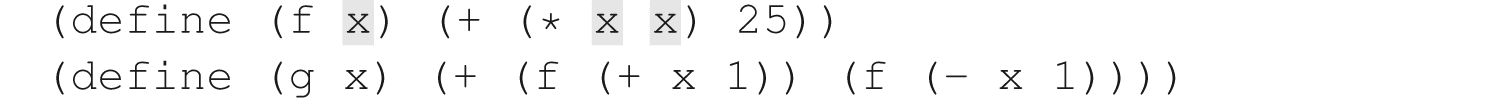
\includegraphics[width=0.85\textwidth]{images/00418.png}
\end{center}

显而易见，函数 \code{f} 中出现的 \code{x} 与函数 \code{g} 中出现的 \code{x} 完全没有任何关系。我们可以系统性地将 \code{f} 中阴影标记的 \code{x} 全部替换为 \code{y}，函数计算出的结果依然毫无二致。简而言之，阴影标记的 \code{x} 仅在 \code{f} 的定义内部拥有意义，而在其他任何地方均不存在。

同时，\code{f} 的函数头中第一次出现的 \code{x} 与其函数体内部出现的 \code{x} 性质完全不同。当我们求值 \code{(f n)} 时，函数名 \code{f} 彻底消失，而函数体内的 \code{x} 则被统一替换为实参 \code{n}。为了区分变量的这两种角色：
\begin{itemize}
  \item 我们将出现在函数头（或形参列表）中的变量称为\term{绑定出现}（binding occurrence）；
  \item 将出现在函数体内部被引用的变量称为\term{约束出现}（bound occurrence）；
  \item 我们称 \code{x} 的绑定出现\textbf{约束}了 \code{f} 体内所有出现的 \code{x}；
  \item 某个绑定出现所管辖并生效的代码区域，被称为其\term{词法作用域}（lexical scope）。
\end{itemize}

上述程序在顶层还绑定了两个名字：\code{f} 和 \code{g}。它们的作用域被称为\term{顶层作用域}（top-level scope）。

反之，若某个变量在所处环境中没有任何绑定出现，它就被称为\term{自由出现}（free occurrence，即自由变量）。自由变量是没有定义的名称——既不是语言内建的，也不是由库引入的，更没有在当前程序中定义。例如在 DrRacket 交互区中分别输入 \code{f}、\code{g} 和 \code{x}：

\begin{replbox}
> f
f
> g
g
> x
x: this variable is not defined
\end{replbox}

词法作用域可以用精巧的箭头图来具象化表示：

\begin{center}
  
\includegraphics[width=0.85\textwidth]{images/00419.png}
\end{center}

\begin{notebox}[DrRacket 的语法检查图示]
点击 DrRacket 右上角的“Check Syntax”（检查语法）按钮，将鼠标悬停在变量上方，DrRacket 会自动绘制出完全一致的词法绑定箭头！
\end{notebox}

图~\ref{fig:00420_toplevel} 展示了顶层作用域的绑定关系：

\begin{center}
  
\includegraphics[width=0.85\textwidth]{images/00420.png}
  \captionof{figure}{顶层作用域绑定关系}\label{fig:00420_toplevel}
\end{center}

\code{f} 的绑定出现带有圆点标记，射出的箭头指向它所有生效的被调用处。这些图示同样精准地解释了变量重命名的本质原理：\textbf{重命名形参，就是找到其词法作用域内的所有约束出现并同步替换}。

\begin{exercise}{绘制词法绑定箭头}{300}
考虑以下简单的 ISL+ 程序：

\begin{center}
  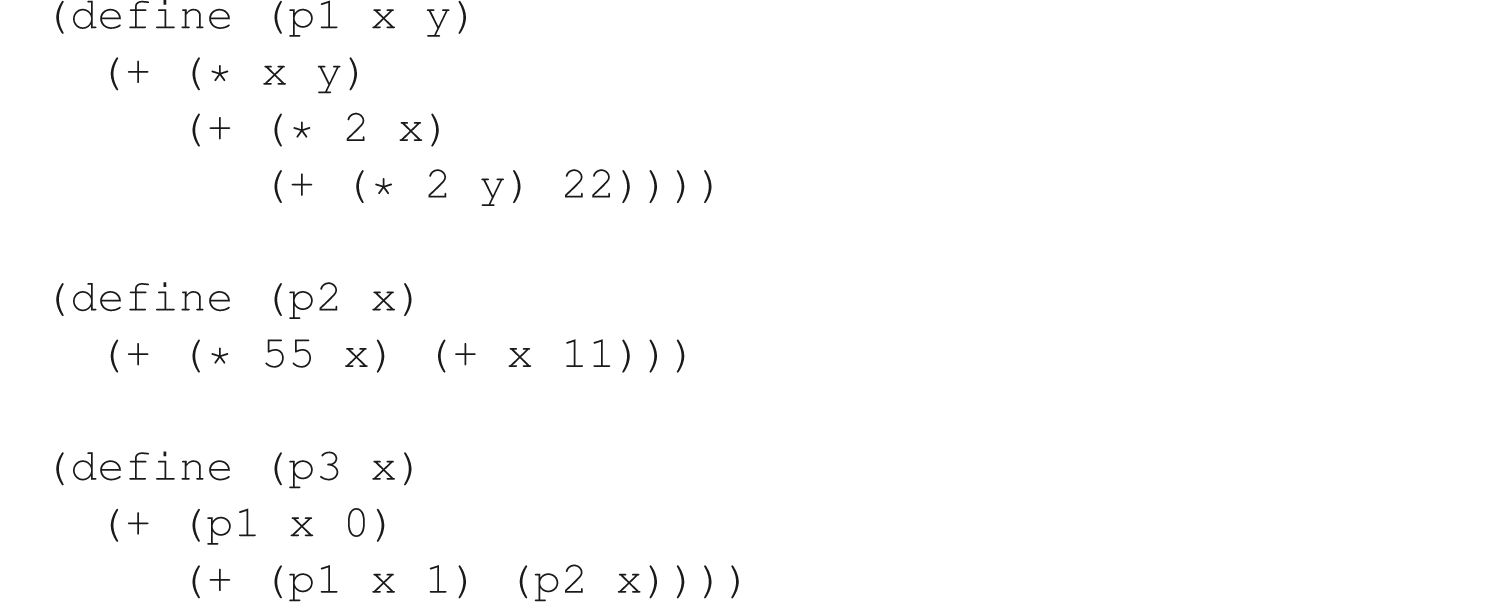
\includegraphics[width=0.85\textwidth]{images/00421.png}
\end{center}

从 \code{p1} 的参数 \code{x} 出发，绘制箭头指向其管辖的所有约束出现。再从 \code{p1} 本身出发，绘制箭头指向所有调用 \code{p1} 的位置。在 DrRacket 中使用“Check Syntax”功能验证你的答案。
\end{exercise}

与全局顶层定义不同，\code{local} 内部定义的可见范围被严格限制：\textbf{局部定义的作用域就是当前所属的整个 \code{local} 表达式}：

\begin{center}
  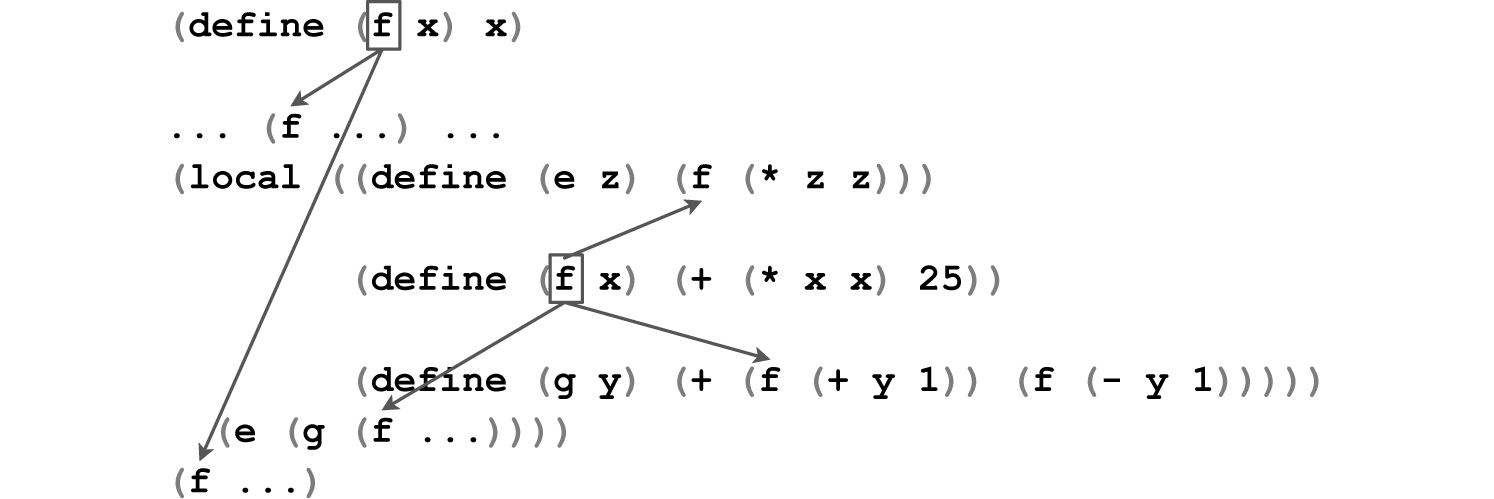
\includegraphics[width=0.85\textwidth]{images/00422.png}
\end{center}

在 \code{local} 之外出现的同名标识符完全不受局部定义的管辖。

由于作用域是一个连续的代码文本区域，计算机科学家常用\term{作用域轮廓框}（scope boxes）来直观界定范围：

\begin{center}
  
\includegraphics[width=0.85\textwidth]{images/00423.png}
\end{center}

对于 \code{local}，方框则包裹住整个 \code{local} 表达式：

\begin{center}
  
\includegraphics[width=0.85\textwidth]{images/00424.png}
\end{center}

借助方框图，我们可以轻易理解当内部局部定义重用了外层的变量名时所发生的\term{变量遮蔽}（shadowing）与\term{作用域空洞}（holes in scope）：

\begin{center}
  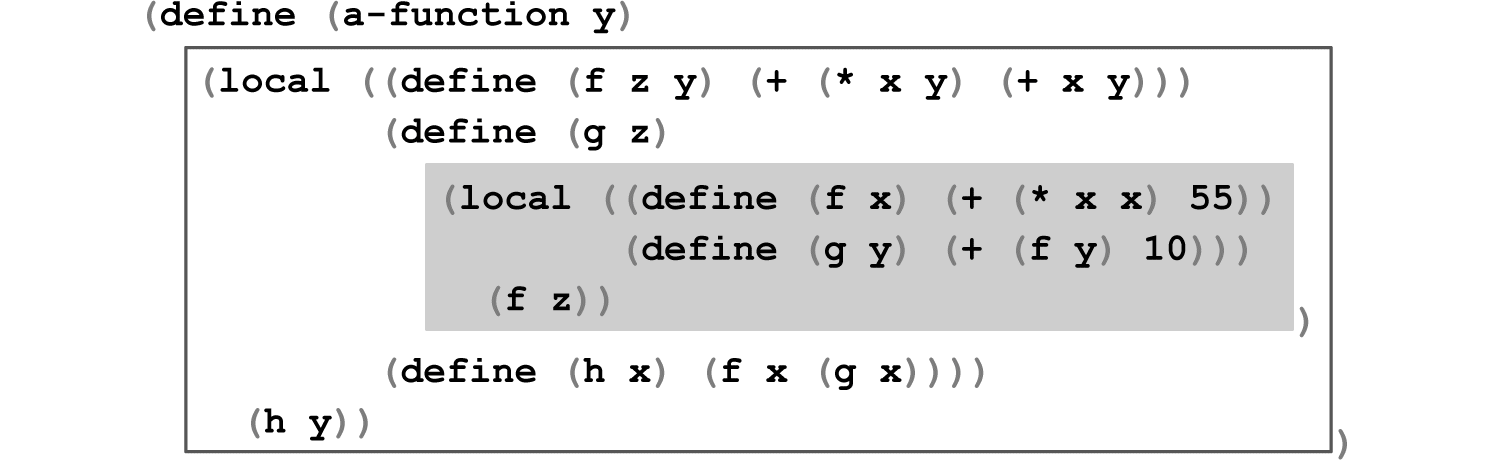
\includegraphics[width=0.85\textwidth]{images/00425.png}
\end{center}

灰色框表示内层 \code{f} 的作用域，白色框表示外层 \code{f} 的作用域。落在灰色框内部的调用一律指向内层定义；只有落在白框且在灰框之外的调用才指向外层定义。灰色框相当于在外层作用域中挖出了一个“空洞”。

在参数命名中同样可能产生空洞：

\begin{center}
  
\includegraphics[width=0.85\textwidth]{images/00426.png}
\end{center}

总体而言，程序的词法作用域始终构成了一套层次分明、逐步嵌套的几何轮廓体系。

\begin{exercise}{为排序程序绘制词法作用域轮廓框}{301}
在图~\ref{fig:105} 中，为 \code{sort} 和 \code{alon} 的每个绑定出现画出作用域方框，并画出从引用指向绑定的箭头。然后在图~\ref{fig:106} 的变体上重复此练习。除了变量名称不同之外，这两个函数的行为有何区别？

\begin{center}
  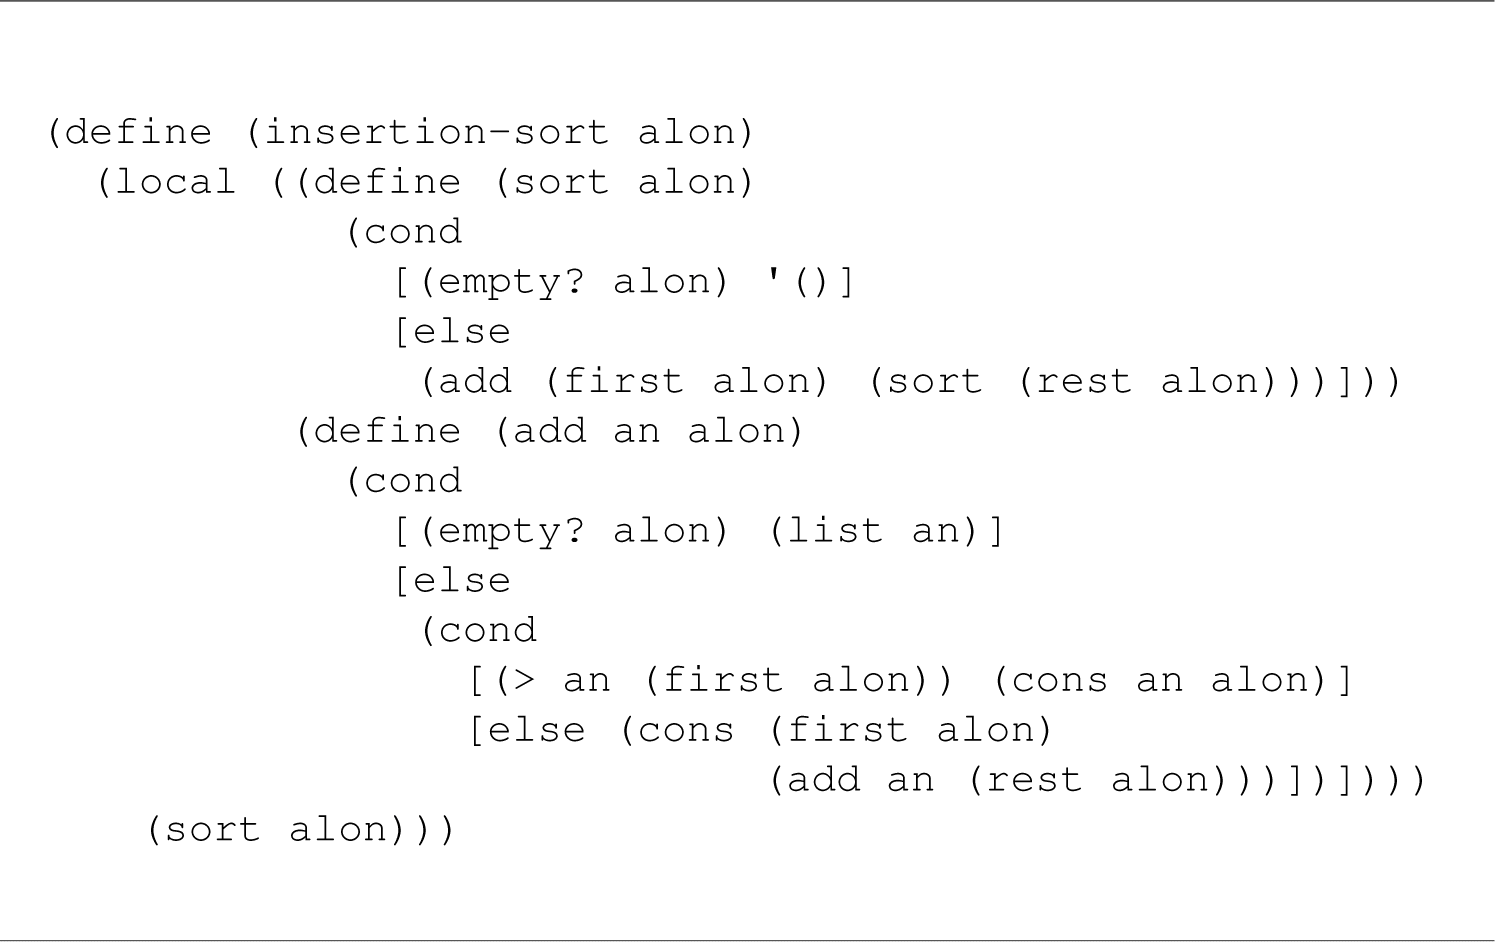
\includegraphics[width=0.85\textwidth]{images/00427.png}
  \captionof{figure}{练习 301 的词法作用域轮廓 (版本 1)}\label{fig:105}
\end{center}

\begin{center}
  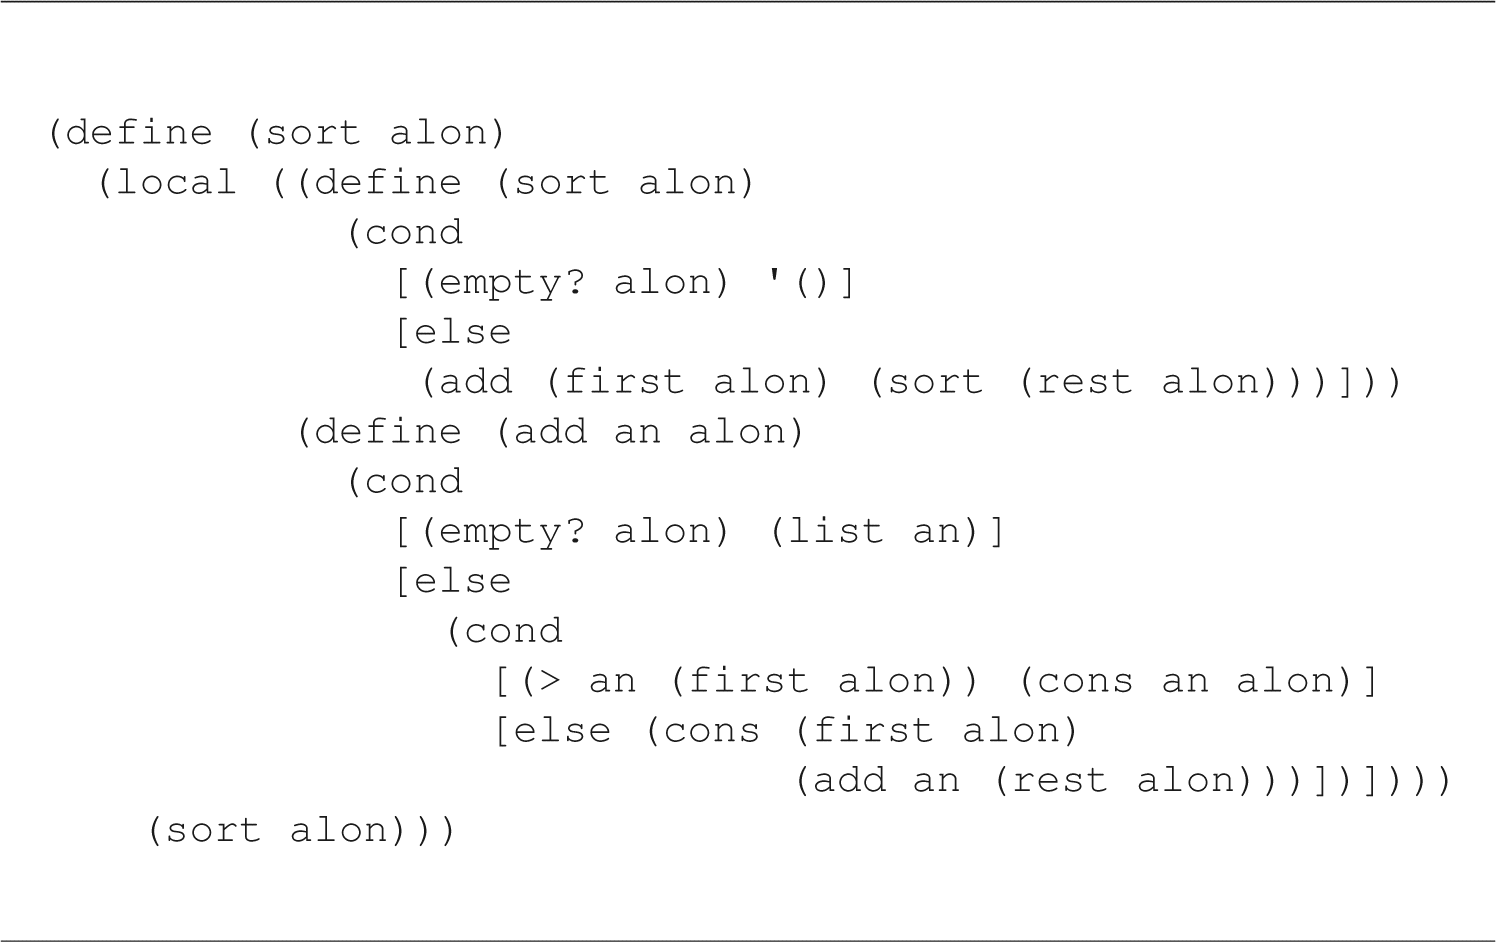
\includegraphics[width=0.85\textwidth]{images/00428.png}
  \captionof{figure}{练习 301 的词法作用域轮廓 (版本 2)}\label{fig:106}
\end{center}
\end{exercise}

\begin{exercise}{常量的自引用陷阱}{302}
回顾每个变量的值均来自于其绑定出现。考虑以下定义：
\begin{lstlisting}[language=BSL]
(define x (cons 1 x))
\end{lstlisting}
右侧阴影中的 \code{x} 在哪里被绑定？既然这是一个普通常量定义而非函数定义，右侧表达式必须被立刻求值。根据求值法则，右侧表达式的值应当是什么？在 DrRacket 中运行会发生什么？
\end{exercise}

对于 \code{lambda} 表达式，其形参的作用域就是其整个函数体表达式：

\begin{center}
  
\includegraphics[width=0.85\textwidth]{images/00429.png}
\end{center}

\begin{exercise}{lambda 表达式中的绑定分析}{303}
在以下三个 \code{lambda} 表达式中，分别从阴影标记的 \code{x} 出发，绘制箭头指向其真正的绑定出现：

\begin{center}
  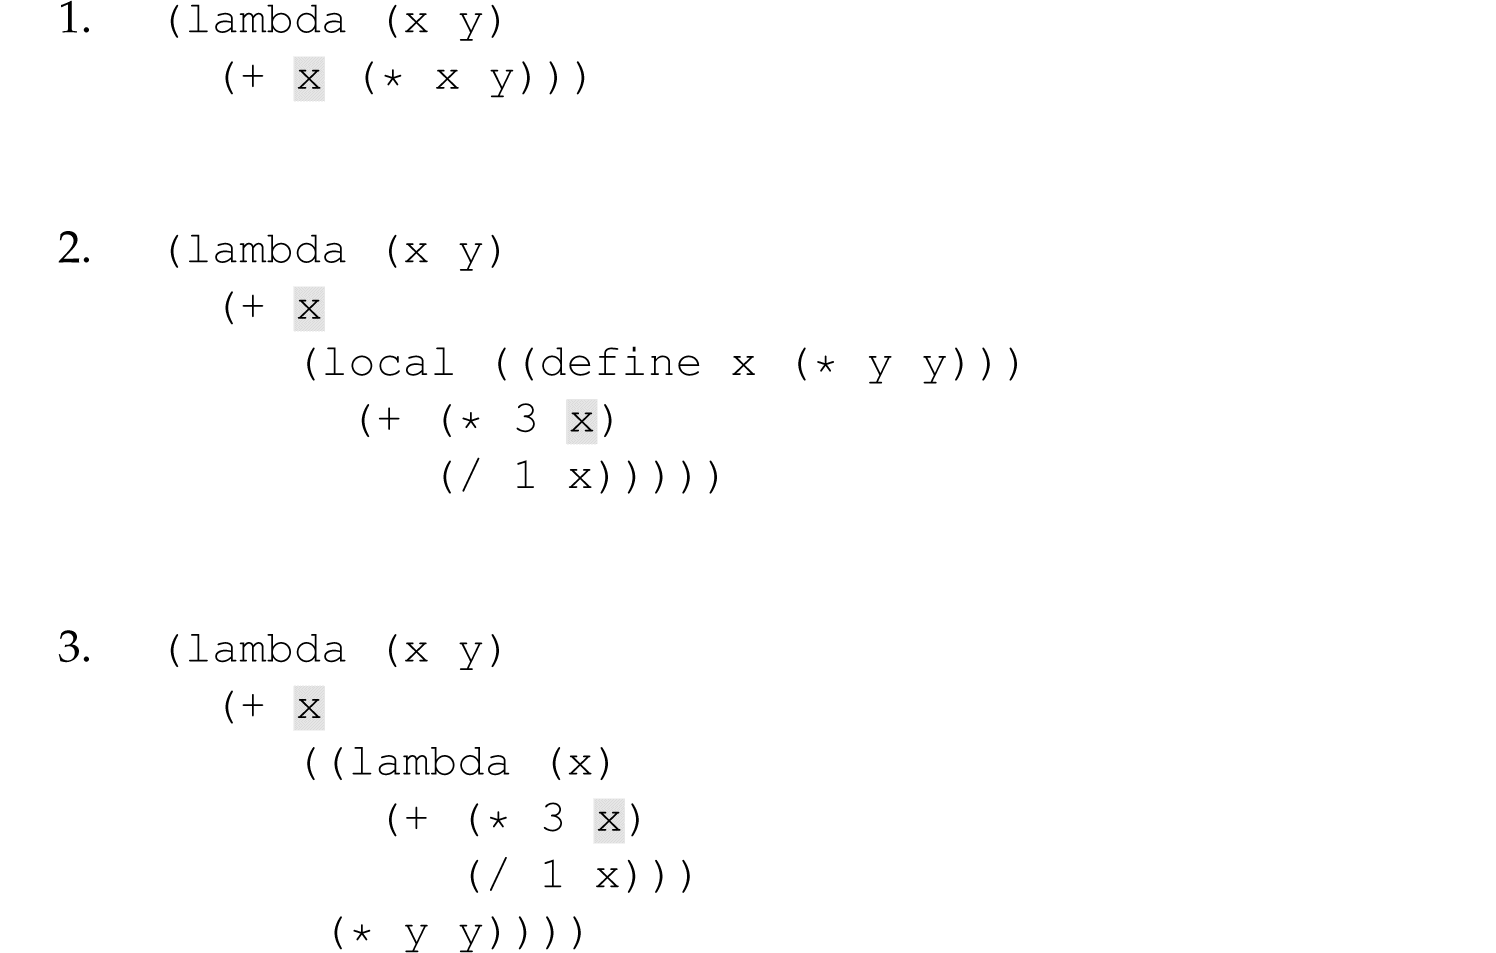
\includegraphics[width=0.85\textwidth]{images/00430.png}
\end{center}

并为每个作用域绘制方框及必要的空洞。
\end{exercise}

% ------------------------------------------------------------------------------
\intermezzosection{ISL 的 for 推导式 (ISL for Loops)}
\label{sec:intermezzo03_loops}

虽然第三部分从未直接使用“循环”这个词，但我们一直在进行循环操作。从本质上说，\term{循环}（loop）就是遍历复合数据并逐一处理其元素，同时合成新的数据结构。例如，\code{map} 遍历列表并收集变换结果；\code{build-list} 遍历自然数区间并构造成新列表。

\begin{notebox}[加载抽象拓展库]
要使用本节介绍的高级循环与模式匹配，请在定义区顶部添加：
\begin{lstlisting}[language=BSL]
(require 2htdp/abstraction)
\end{lstlisting}
\end{notebox}

ISL+ 中的循环与传统命令式语言有着根本不同：传统循环往往通过副作用修改内存，而不直接产出新的复合数据；而 ISL+ 的循环专注于\textbf{纯函数式的数据变换与聚合}。此外，语法形式的循环相比纯函数组合具有两大优势：首先，其语法结构能更加醒目地表达编程意图；其次，编译器通常能将语法循环优化为速度更快的底层机器指令。

图~\ref{fig:107} 给出了扩展的 for 推导式文法：

\begin{center}
  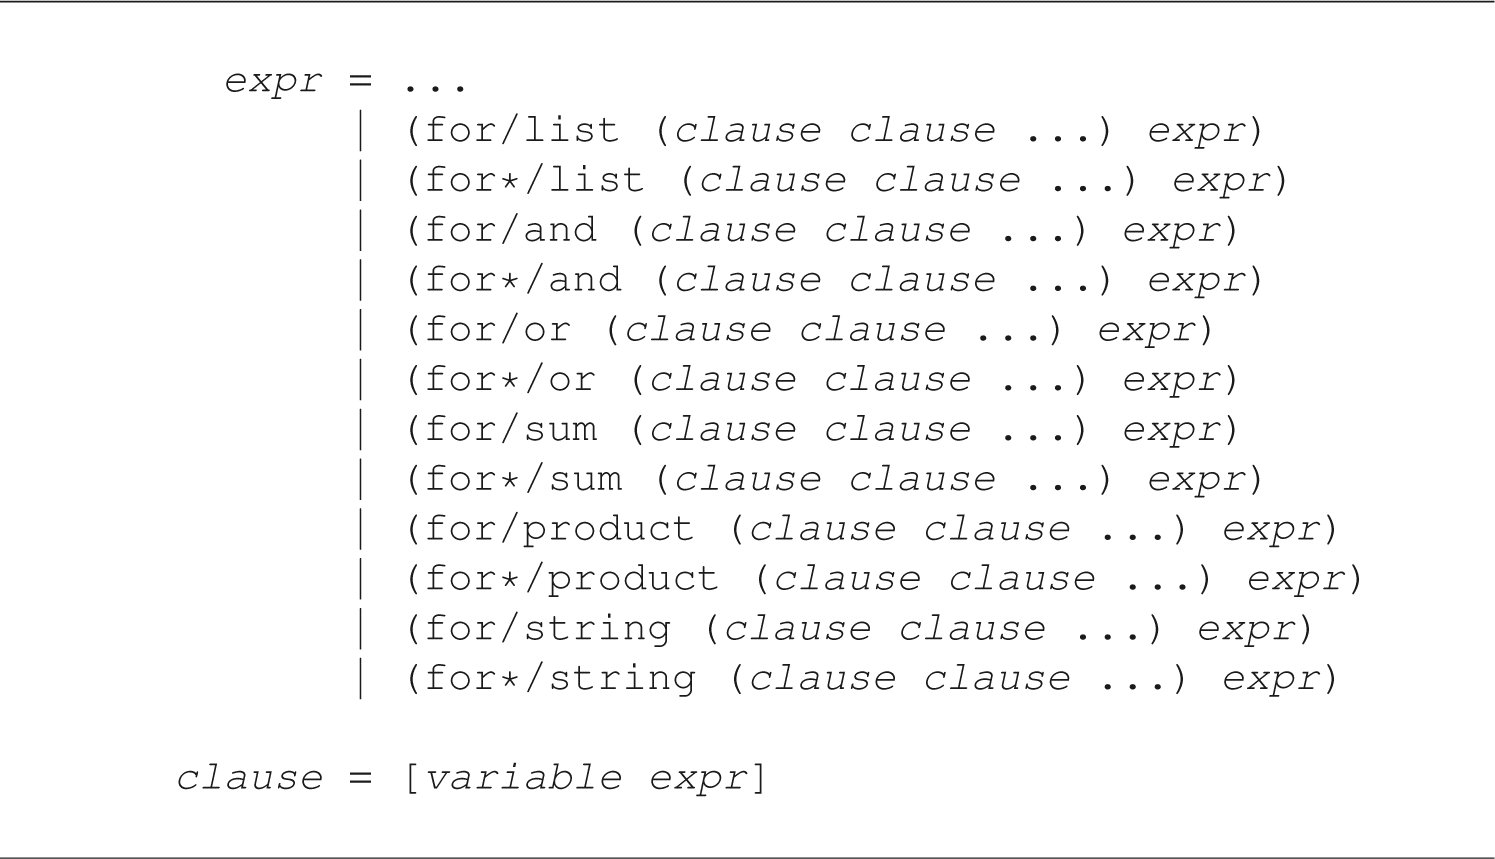
\includegraphics[width=0.85\textwidth]{images/00431.png}
  \captionof{figure}{ISL+ 拓展的 for 推导式文法}\label{fig:107}
\end{center}

文法清晰地呈现出成对出现的六组循环构造：\code{for} 与 \code{for*}，分别对应于 \code{list}、\code{and}、\code{or}、\code{sum}、\code{product} 和 \code{string}。

两者的核心区别在于\textbf{词法作用域与遍历维度}：
\begin{itemize}
  \item \code{for} 形式是\textbf{并行遍历}（parallel traversal），各子句中的序列同时前进一步，且后续子句\textbf{不能}引用前面子句引入的循环变量；
  \item \code{for*} 形式是\textbf{嵌套笛卡尔积遍历}（nested traversal），类似多重嵌套循环，且后续子句\textbf{可以}自由引用前面子句绑定的循环变量！
\end{itemize}

\begin{center}
  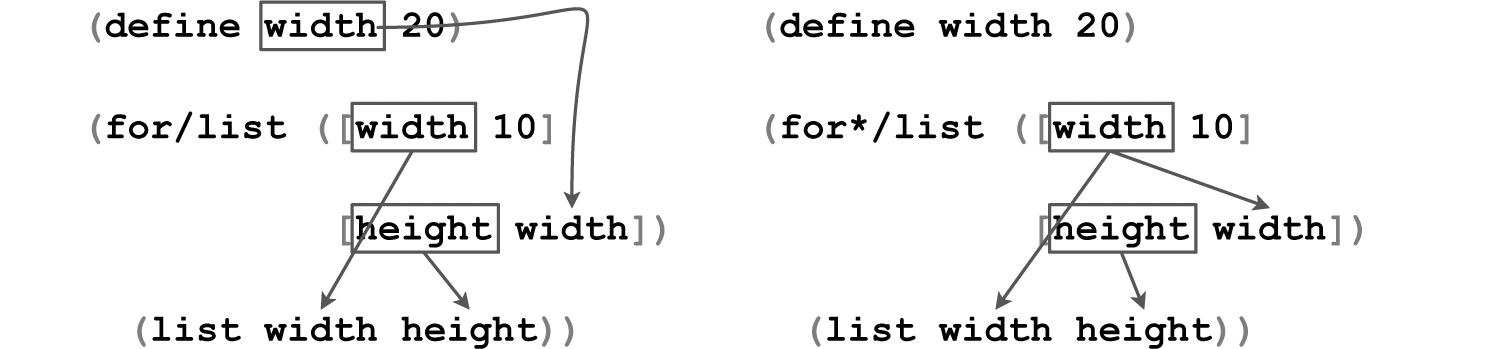
\includegraphics[width=0.85\textwidth]{images/00432.png}
\end{center}

\code{for/list} 的语义极其简洁自然：
\begin{replbox}
> (for/list ([i 10]) i)
(list 0 1 2 3 4 5 6 7 8 9)
\end{replbox}
这直接等价于 \code{(build-list 10 (lambda (i) i))}！

两个序列的并行拉链组合（zip）：
\begin{center}
  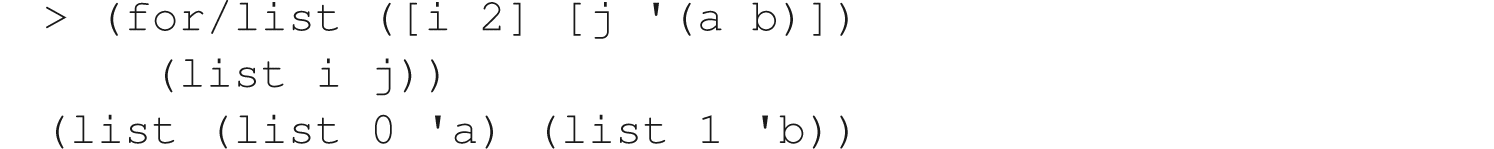
\includegraphics[width=0.85\textwidth]{images/00433.png}
\end{center}
对比纯函数式的写法（图~\ref{fig:00434_zip_plain}），\code{for/list} 展现出了惊人的可读性：
\begin{center}
  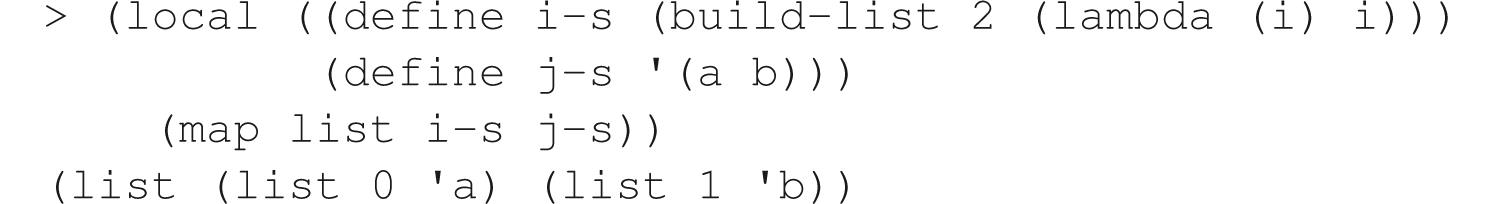
\includegraphics[width=0.85\textwidth]{images/00434.png}
  \captionof{figure}{列表组合处理代数形式}\label{fig:00434_zip_plain}
\end{center}

\begin{notebox}[样例问题：设计 enumerate 函数]
设计函数 \code{enumerate}，接收一个列表，产生由每个元素与其对应的索引编号组成的二元对列表。
\end{notebox}

借助 \code{for/list}，解法极其优雅自然：
\begin{lstlisting}[language=BSL]
; [List-of X] -> [List-of [List N X]]
(check-expect (enumerate '(a b c)) '((1 a) (2 b) (3 c)))
(define (enumerate lx)
  (for/list ([x lx] [ith (length lx)])
    (list (+ ith 1) x)))
\end{lstlisting}

相比之下，\code{for*/list} 则展开为嵌套循环（笛卡尔积）：

\begin{center}
  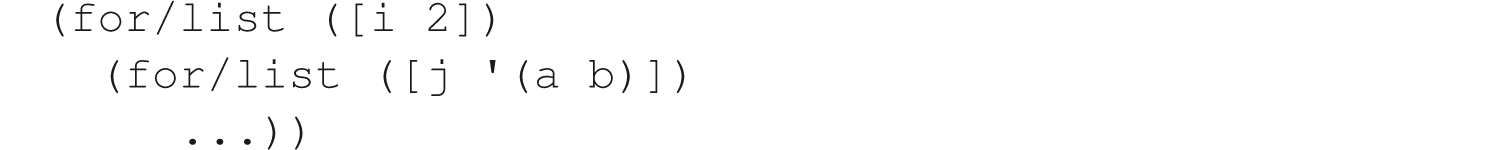
\includegraphics[width=0.85\textwidth]{images/00435.png}
\end{center}

\begin{exercise}{对比 for/list 与 for*/list}{304}
在 DrRacket 交互区中分别求值：
\begin{lstlisting}[language=BSL]
(for/list ([i 2] [j '(a b)]) (list i j))
(for*/list ([i 2] [j '(a b)]) (list i j))
\end{lstlisting}
对比两者的输出结构差异。
\end{exercise}

图~\ref{fig:00436_interaction}、\ref{fig:00437_table} 和 \ref{fig:00438_nest} 详细演示了两者在多子句依赖下的行为细节：

\begin{center}
  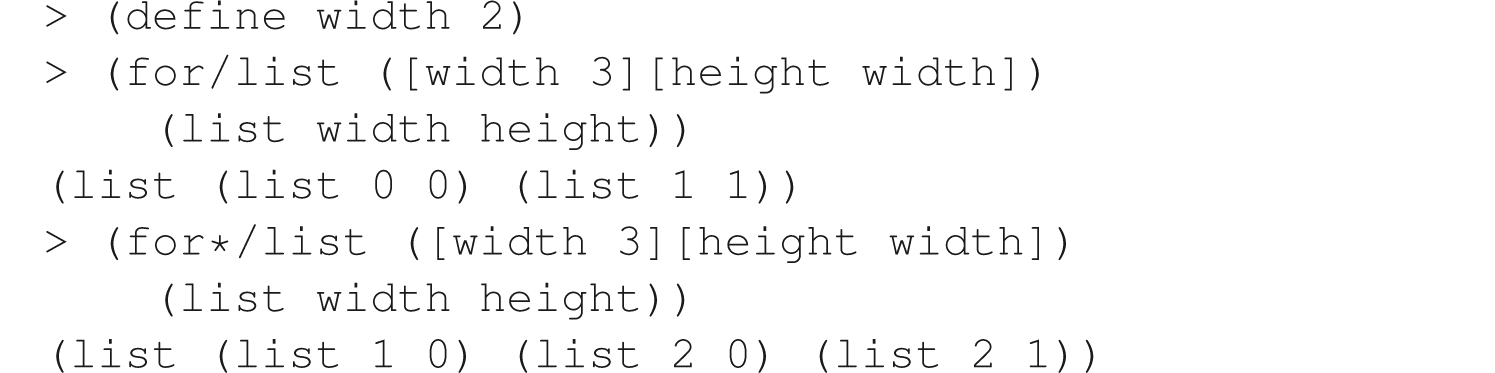
\includegraphics[width=0.85\textwidth]{images/00436.png}
  \captionof{figure}{语法结构交互分析}\label{fig:00436_interaction}
\end{center}

\begin{center}
  
\includegraphics[width=0.85\textwidth]{images/00437.png}
  \captionof{figure}{语法结构对照表}\label{fig:00437_table}
\end{center}

\begin{center}
  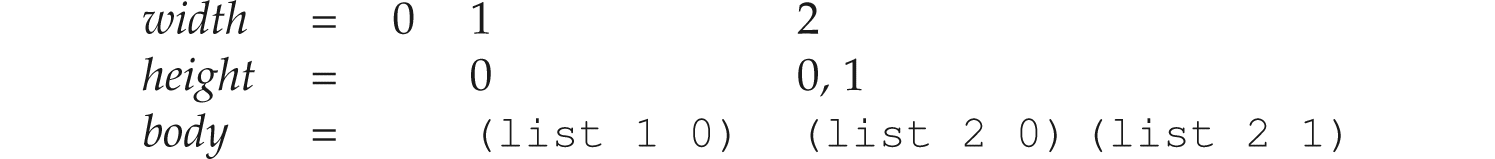
\includegraphics[width=0.85\textwidth]{images/00438.png}
  \captionof{figure}{嵌套语法分析}\label{fig:00438_nest}
\end{center}

借助 \code{for*/list}，计算两个列表的笛卡尔乘积函数 \code{cross} 可以轻松写出：

\begin{center}
  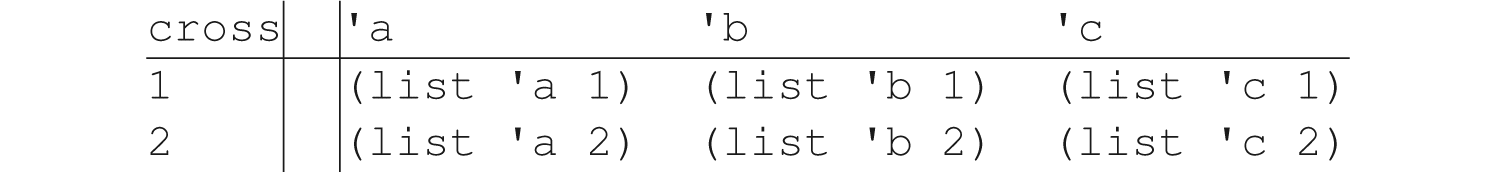
\includegraphics[width=0.85\textwidth]{images/00439.png}
\end{center}

\begin{center}
  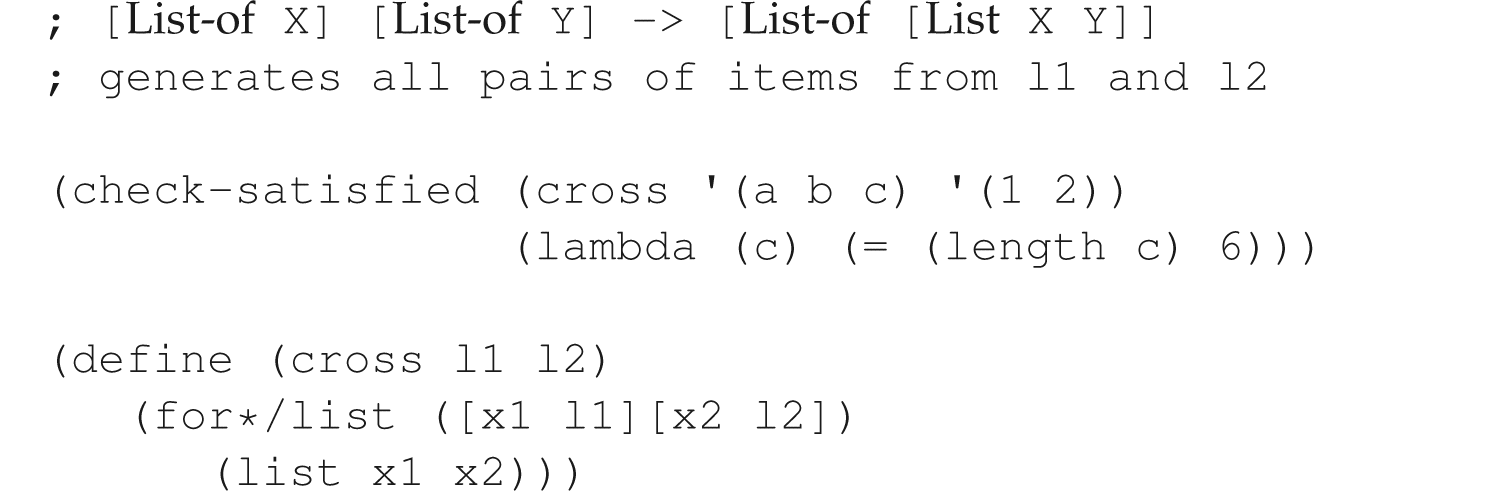
\includegraphics[width=0.85\textwidth]{images/00440.png}
\end{center}

图~\ref{fig:108} 更是展现了抽象的无上威力：仅用 5 行代码，通过 \code{for*/list} 搞定了第 12.4 节极为复杂的字母全排列生成算法！

\begin{center}
  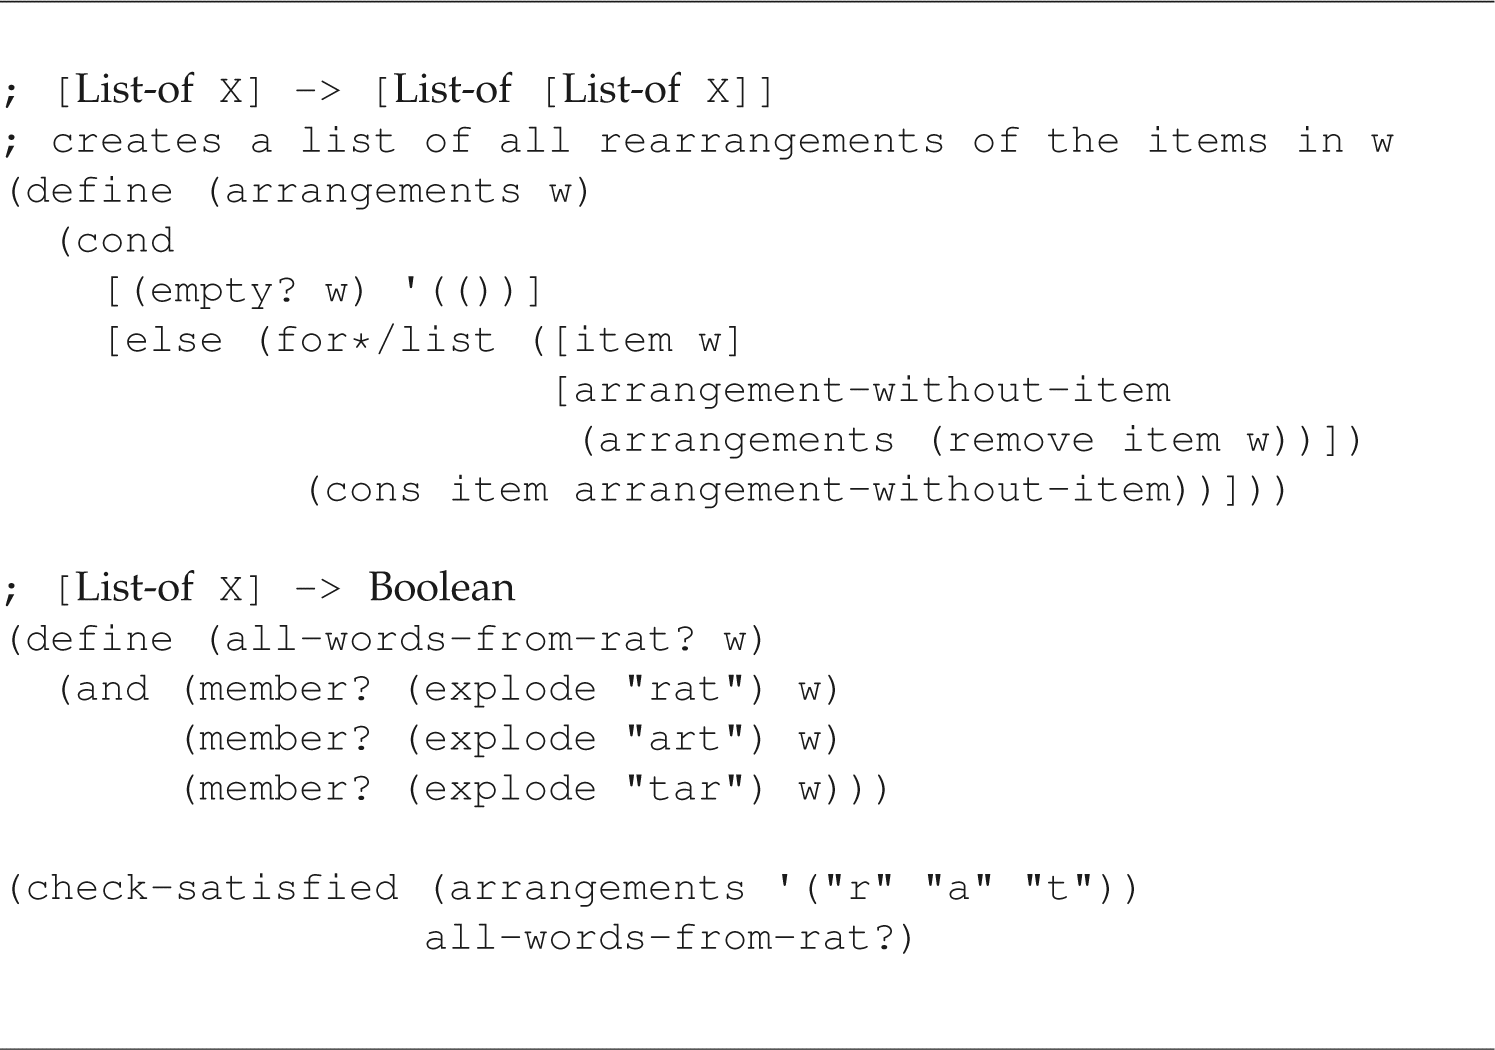
\includegraphics[width=0.85\textwidth]{images/00441.png}
  \captionof{figure}{利用 for*/list 紧凑实现的字母全排列程序}\label{fig:108}
\end{center}

其他循环变体同样顾名思义：
\begin{itemize}
  \item \code{for/and}：用 \code{and} 汇聚所有迭代结果；
  \item \code{for/or}：用 \code{or} 汇聚，返回首个非假值；
  \item \code{for/sum}：将每次迭代计算出的数值求和；
  \item \code{for/product}：将每次迭代的值累乘；
  \item \code{for/string}：将单字符拼接为新字符串。
\end{itemize}

配合图~\ref{fig:109} 中的无限自然数发生器 \code{in-naturals} 和步长发生器 \code{in-range}，循环的能力进一步大放异彩：

\begin{center}
  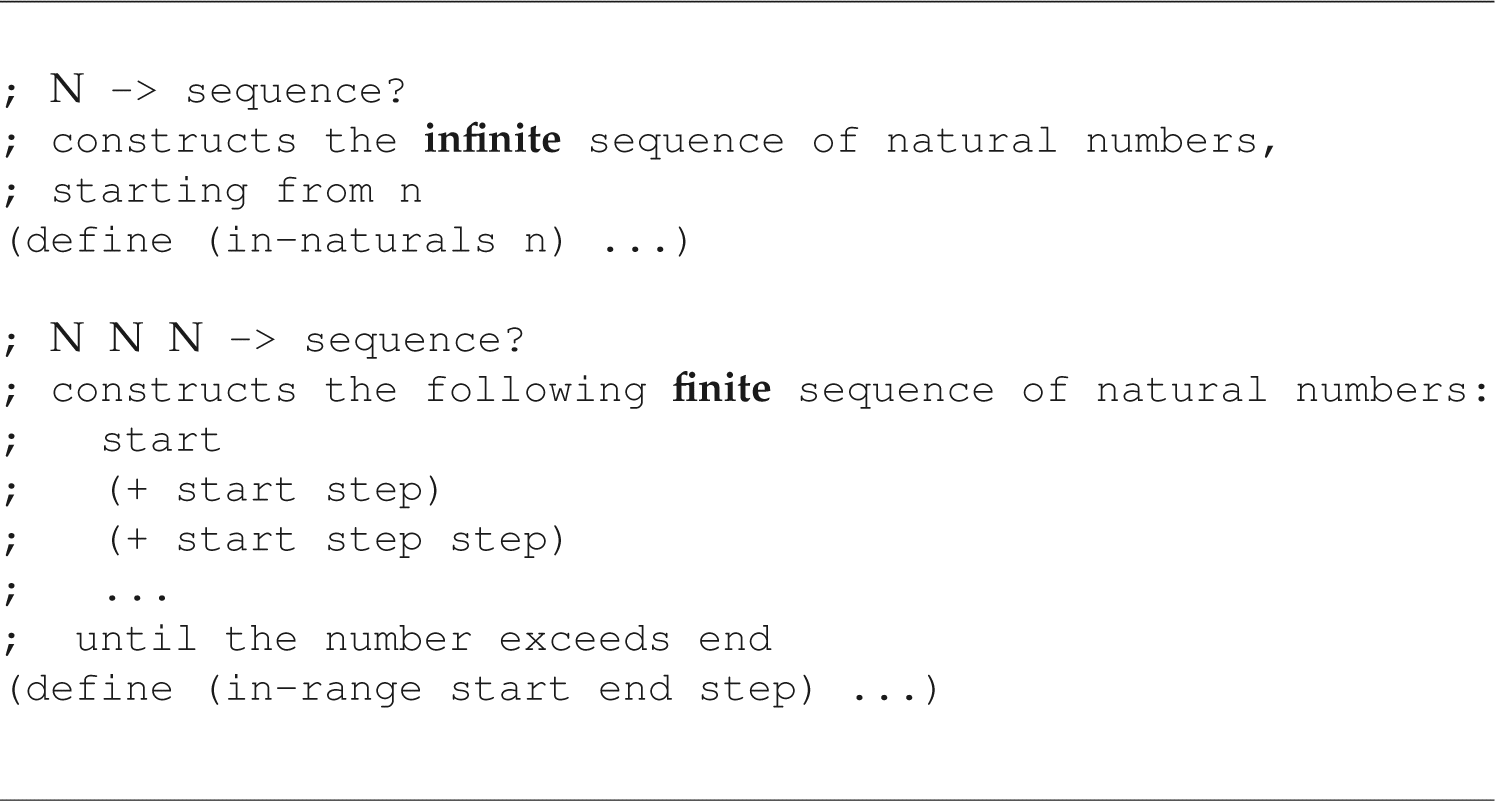
\includegraphics[width=0.85\textwidth]{images/00442.png}
  \captionof{figure}{构造自然数序列的高级生成器}\label{fig:109}
\end{center}

例如简洁定义求前 $n$ 个偶数和的函数：
\begin{lstlisting}[language=BSL]
; N -> Number
(define (sum-evens n)
  (for/sum ([i (in-range 0 n 2)]) i))
\end{lstlisting}

\begin{exercise}{使用循环重构 convert-euro}{305}
使用 \code{for/list} 重新实现练习 267 中的货币转换函数 \code{convert-euro}。
\end{exercise}

\begin{exercise}{使用循环生成各类列表}{306}
使用 \code{for/list} 分别实现：
\begin{enumerate}
  \item 生成列表 \code{(list 0 ... (- n 1))}；
  \item 生成列表 \code{(list 1 ... n)}；
  \item 生成列表 \code{(list 1 1/2 ... 1/n)}；
  \item 生成前 $n$ 个偶数列表；
  \item 重新实现练习 262 中的单位对角方阵 \code{identityM}。
\end{enumerate}
最后，使用 \code{for/list} 重新实现练习 250 中的制表函数 \code{tabulate}。
\end{exercise}

\begin{exercise}{使用 for/or 查找名字}{307}
使用 \code{for/or} 定义 \code{find-name}，检索列表中首个匹配前缀的名字。并定义一个函数，确保列表中没有名字的长度超过给定宽度。
\end{exercise}

% ------------------------------------------------------------------------------
\intermezzosection{模式匹配 (Pattern Matching)}
\label{sec:intermezzo03_match}

当我们为具有多个分支的数据定义设计函数时，传统做法是使用多分支的 \code{cond} 表达式：在每个分支中用类型谓词进行判定，若匹配成功，再使用大量的\textbf{选择器}（selectors）层层拆解复合数据。前三部分反复练习了这一流程。

然而，重复的代码模式呼唤着语言级的抽象！函数式编程语言的设计者们引入了\term{模式匹配}（Pattern Matching，在 ISL+ 中表现为 \code{match} 表达式），将类型判定谓词与字段提取选择器完美融为一体。

图~\ref{fig:110} 给出了 \code{match} 的文法规范：

\begin{center}
  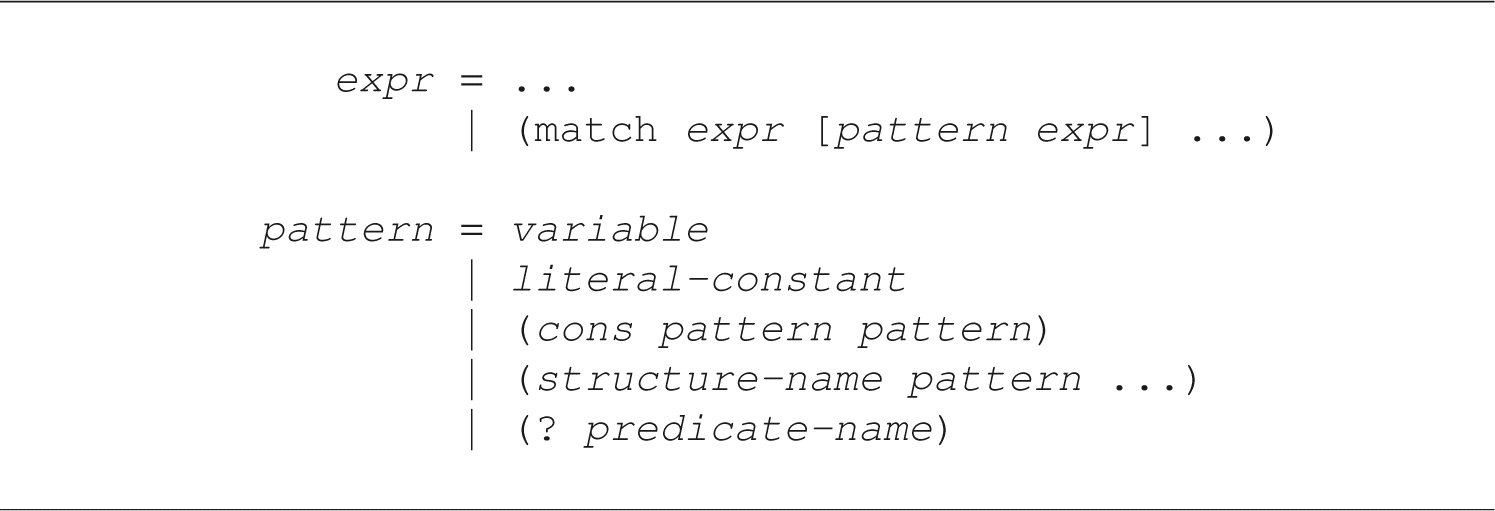
\includegraphics[width=0.85\textwidth]{images/00443.png}
  \captionof{figure}{ISL+ 模式匹配表达式文法}\label{fig:110}
\end{center}

\begin{lstlisting}[language=BSL]
(match expr
  [pattern1 expr1]
  [pattern2 expr2]
  ...)
\end{lstlisting}

与 \code{cond} 最根本的区别在于：\textbf{\code{match} 的每个模式分支都会开辟一个独立的词法作用域}！模式中出现的变量会自动绑定到被解构数据对应的组成字段上，并在该分支的表达式内部生效：

\begin{center}
  
\includegraphics[width=0.85\textwidth]{images/00444.png}
\end{center}

模式匹配支持极其丰富的解构语法：
\begin{itemize}
  \item \textbf{字面量常量}：仅匹配相等的具体常量；
\begin{center}
  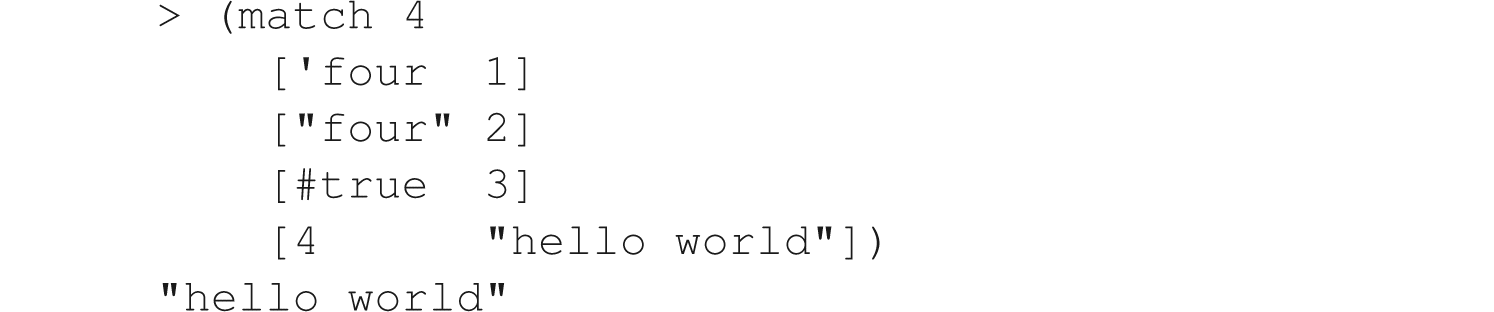
\includegraphics[width=0.85\textwidth]{images/00445.png}
\end{center}
  \item \textbf{变量模式}：匹配任意值，并将其绑定到该变量名上；
\begin{center}
  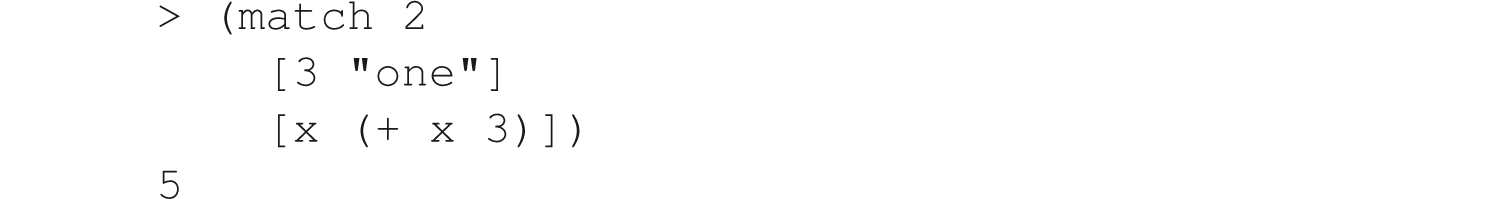
\includegraphics[width=0.85\textwidth]{images/00446.png}
\end{center}
  \item \textbf{\code{(cons p1 p2)} 列表模式}：直接解构列表的首项与剩余部分；
\begin{center}
  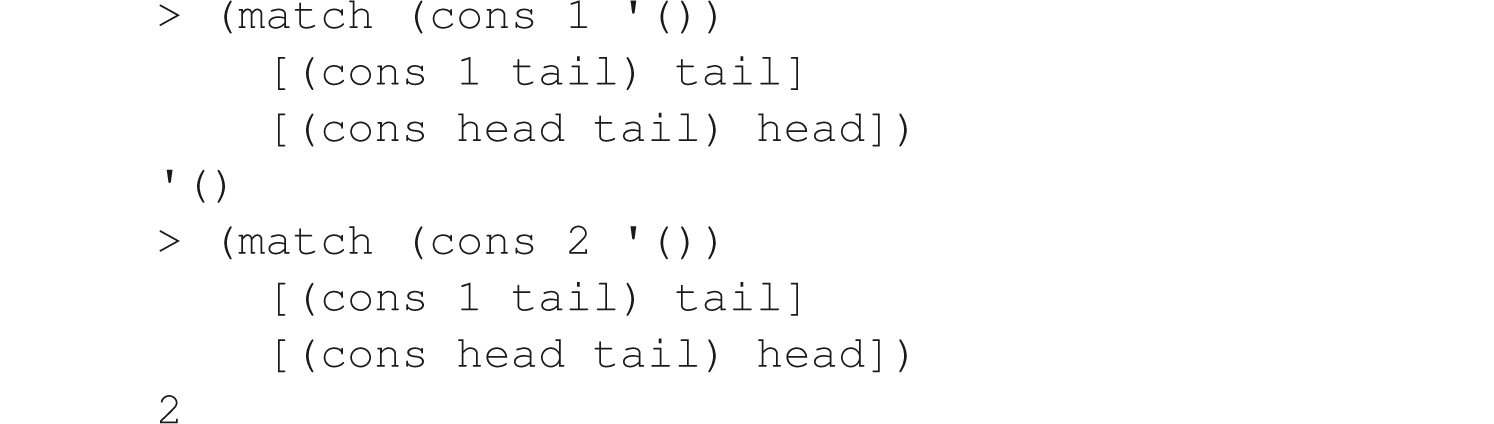
\includegraphics[width=0.85\textwidth]{images/00447.png}
\end{center}
  \item \textbf{结构体模式 \code{(struct-name p1 ... pn)}}：直接解构结构体的各个字段：
\begin{lstlisting}[language=BSL]
(define p (make-posn 3 4))
(match p
  [(posn x y) (sqrt (+ (sqr x) (sqr y)))]) ; 结果为 5
\end{lstlisting}
  \item \textbf{多层深度嵌套模式}：单次匹配即可穿透多层复合结构：
\begin{lstlisting}[language=BSL]
(match (cons (make-phone 713 664 9993) '())
  [(cons (phone area-code 664 9993) tail)
   area-code]) ; 直接提取出 713
\end{lstlisting}
  \item \textbf{谓词模式 \code{(? pred)}}：当且仅当 \code{(pred v)} 为真时匹配。
\end{itemize}

让我们通过真实问题领略 \code{match} 的非凡魅力：

\begin{notebox}[样例 1：获取非空列表的末尾元素]
\begin{lstlisting}[language=BSL]
; [Non-empty-list X] -> X
; 获取非空列表 ne-l 的最后一个元素
(check-expect (last-item '(a b c)) 'c)
(define (last-item ne-l)
  (match ne-l
    [(cons lst '()) lst]
    [(cons fst rst) (last-item rst)]))
\end{lstlisting}
\end{notebox}
无需调用任何 \code{empty?}、\code{cons?}、\code{first}、\code{rest}，模式直接镜像了数据定义本身！

\begin{notebox}[样例 2：俄罗斯套娃层数计算]
\begin{lstlisting}[language=BSL]
; RD.v2 -> N
(define (depth a-doll)
  (match a-doll
    ["doll" 0]
    [(layer c inside) (+ (depth inside) 1)]))
\end{lstlisting}
\end{notebox}

图~\ref{fig:00448_moveright} 展示了太空战游戏中向右平移目标坐标的完整实现：

\begin{center}
  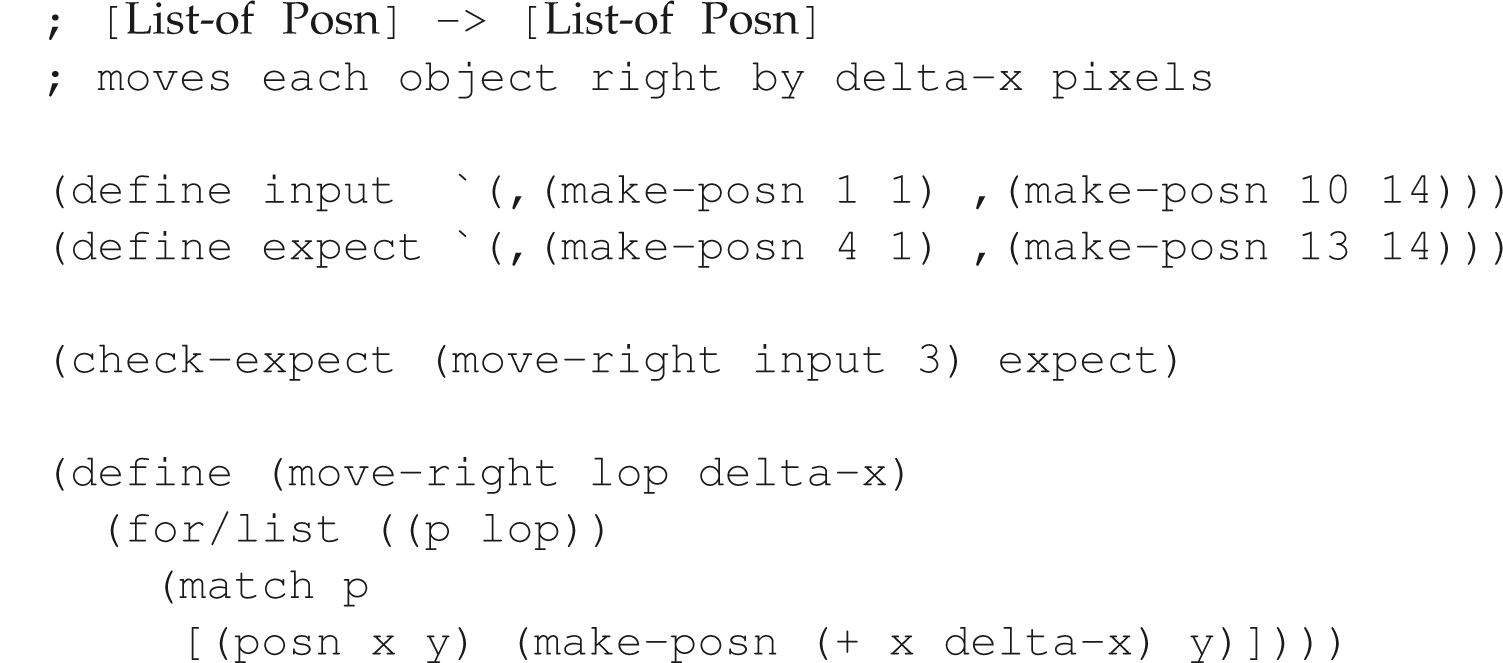
\includegraphics[width=0.85\textwidth]{images/00448.png}
  \captionof{figure}{太空战舰游戏向右移动实现}\label{fig:00448_moveright}
\end{center}

\begin{exercise}{更新电话号码区号}{308}
使用 \code{match} 设计函数 \code{replace}，将电话记录列表中所有区号为 713 的号码替换为 281。
\end{exercise}

\begin{exercise}{统计嵌套行中的词数}{309}
使用 \code{match} 设计函数 \code{words-on-line}，计算由字符串列表构成的列表中每行的单词数量。
\end{exercise}
